\documentclass[12pt]{article}
\usepackage[utf8]{inputenc}
\usepackage[czech]{babel}
\usepackage[plainpages=false,pdfpagelabels,unicode]{hyperref}
\usepackage[pdftex]{graphicx}
\usepackage[margin=2cm, includefoot]{geometry}
\usepackage{bm}

\begin{document}

\title{Praktikum z fyziky plazmatu \\
Studium elektronové koncentrace plazmatu mikrovlnou metodou}
\author{Pavel Ondračka}
\maketitle

\section{Úvod}
Koncentrace elektronů byla určena rezonátorovou metodou, která spočívá v~měření komplexní vysokofrekvenční vodivosti plazmatu.
Relativní permitivita plazmatu $\epsilon_p$ závisí na plazmové elektronové frekvenci $\omega_{pe}$ 

\begin{equation}
\epsilon_p = 1 - \frac{\omega_{pe}^2}{\omega_0^2} \, \mathrm{.}
\end{equation}
Čtverec plazmové frekvence je přímo úměrný elektronové koncentraci
\begin{equation}
\omega_{pe}^2 = \frac{n_e e^2}{\epsilon_0 m_e}  \, \mathrm{.}
\end{equation}
Pro relativní permitivitu materiálu vloženého do rezonátoru platí (následující vzorce předpokládají, že rezonátor pracuje s videm TM$_{010}$):
\begin{equation}
\epsilon_r = \frac{0,271}{0,64} \frac{R^2}{R'^2} \frac{\Delta f}{f_0} + 1 \, \mathrm{,}
\end{equation}
kde $R$ je vnitřní poloměr rezonátoru a $R'$ je poloměr výbojové trubice, $f_0$ je rozonanční frekvence prázdného rezonátoru, $f$ je rozonanční frekvence rezonátoru s výbojem.

Elektronovou koncentraci poté můžeme vypočítat dvěma způsoby. Pokud známe geometrické parametry rezonátoru a výbojové trubice, můžeme koncentraci vypočítat přímo
%
\begin{equation}
n_\mathrm{e} = \frac{0,271}{0,64} \frac{r_0^2}{R^2} \Delta f \frac{8 \pi^2 \epsilon_0 m_\mathrm{e} f_0}{e^2} \, \mathrm{.}
\end{equation}
%
Pokud je neznáme, nebo neznáme přesně vid, který v~rezonátoru převažuje, můžeme použít relativní metodu, kde prvně změříme změnu rezonance $\Delta f_\mathrm{ref}$ při vložení materiálu se známou permitivitou $\epsilon_\mathrm{ref}$ a z té následně určíme permitivitu (a elektronovou koncentraci plazmatu)
\begin{equation}
n_\mathrm{e} = (\epsilon_\mathrm{ref}-1) \frac{\Delta f}{\Delta f_\mathrm{ref}} \frac{4 \pi^2 \epsilon_0 m_\mathrm{e} f_0^2}{e^2} \, \mathrm{.}
\end{equation}

\begin{figure}[htbp]
\begin{center}
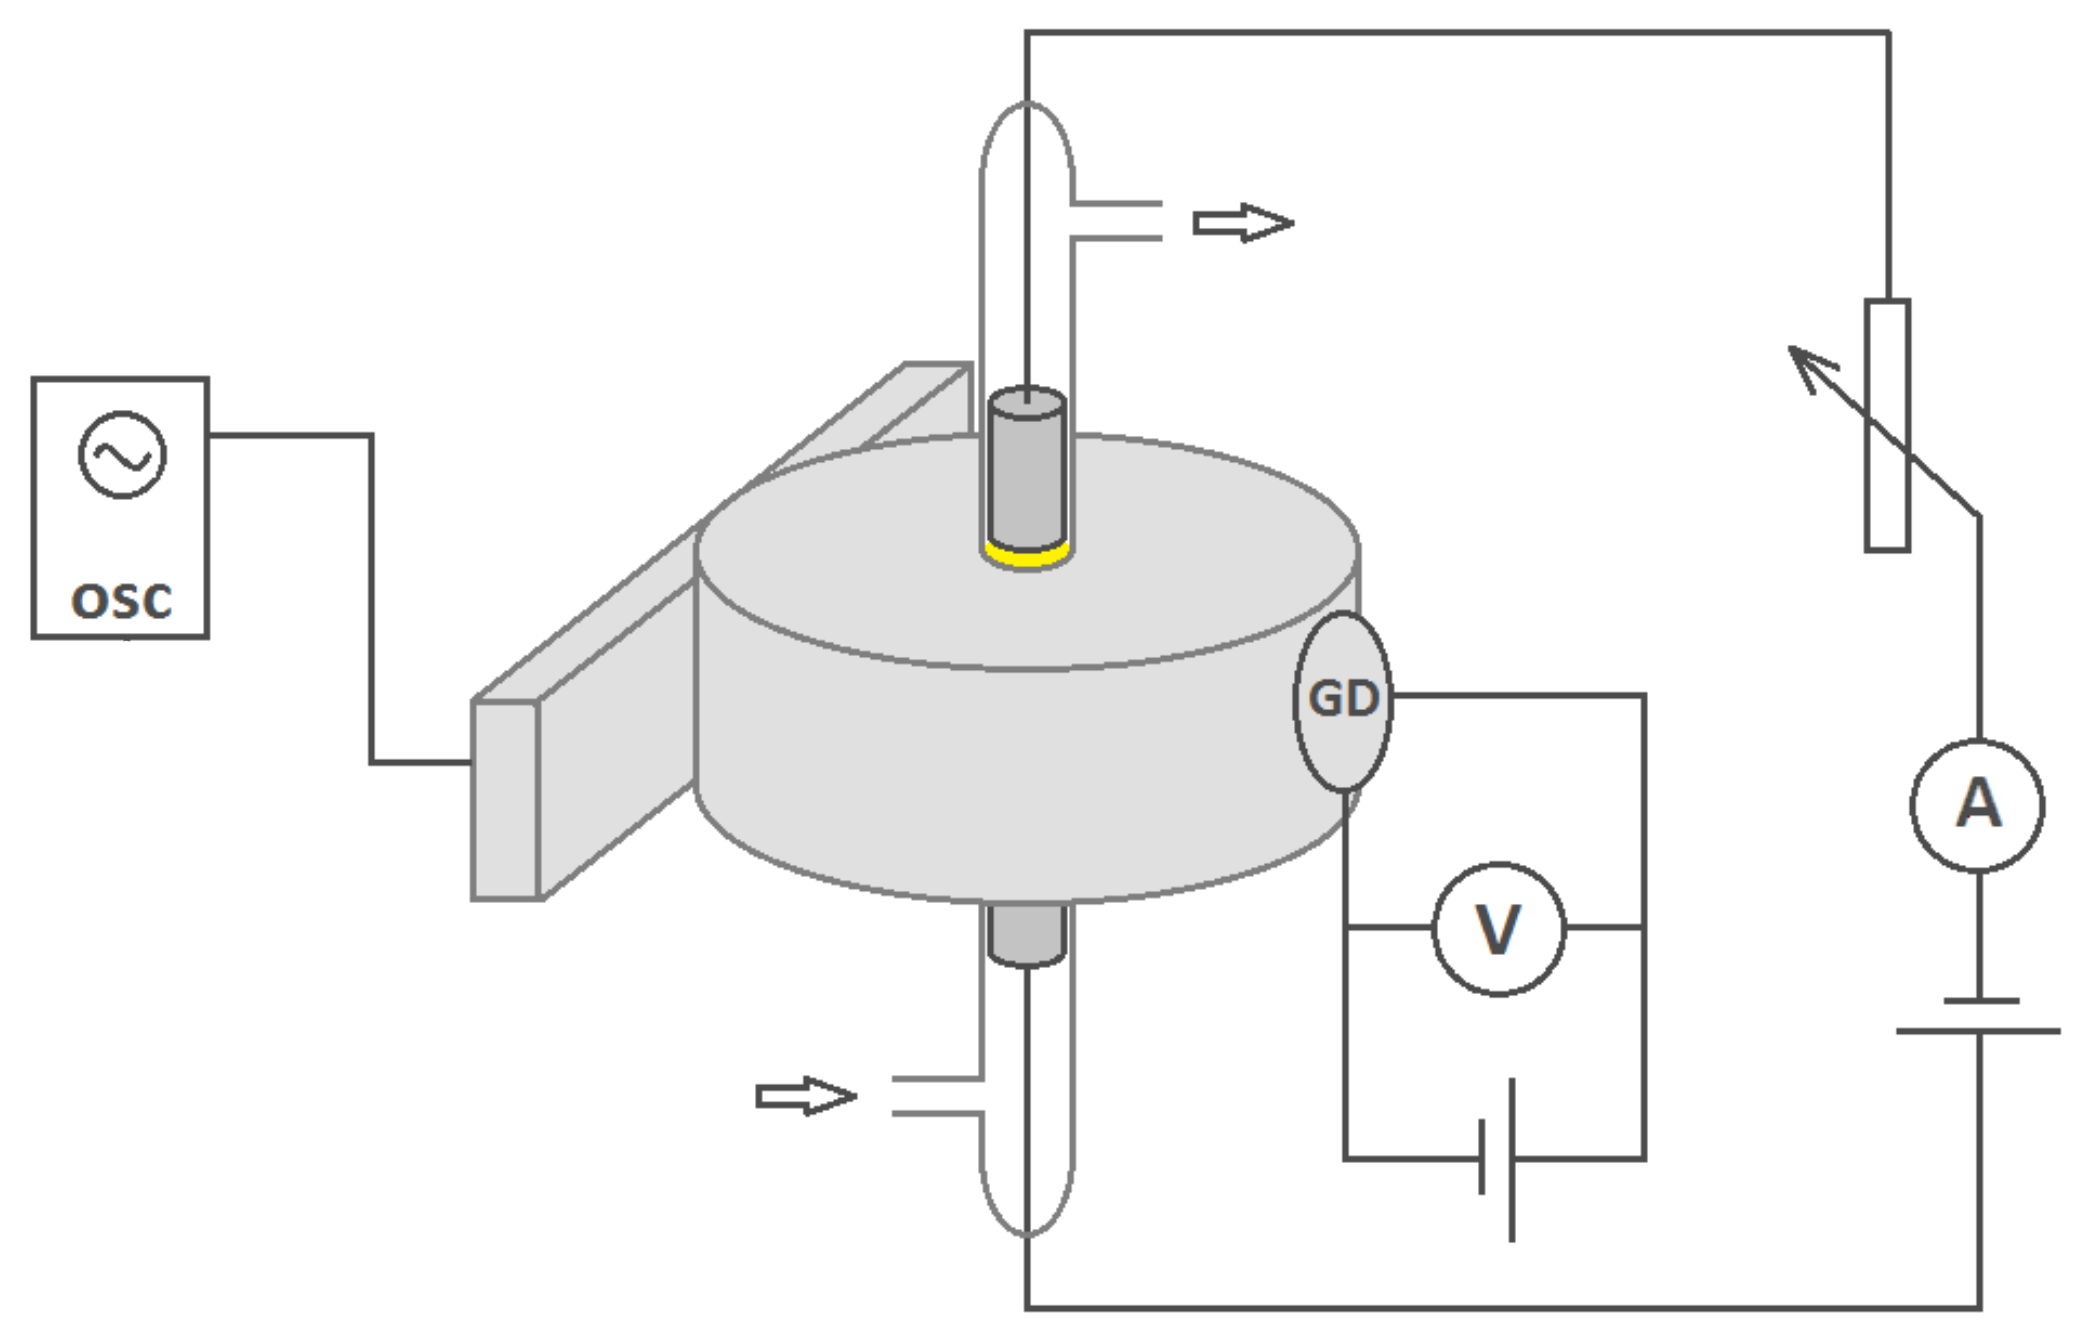
\includegraphics[width=10cm]{schema.png}
\caption{Schéma aparatury, GD -- Gunnova dioda, OSC -- osciloskop}
\label{schema}
\end{center}
\end{figure}

\section{Měření}
Měření bylo prováděno pro tři hodnoty tlaků: 50\,Pa, 100\,Pa a 200\,Pa. Pro tlak 500\,Pa se již výboj nepodařilo zapálit. Byla měřena závislost změny rezonanční frekvence na výbojovém proudu, ze změny rezonanční frekvence byla následně vypočítána elektronová koncentrace. Vnitřní poloměr rezonátoru je $R$ = 3\,cm a vnitřní poloměr výbojové trubice je $R'$ = 4\,mm. Naměřené hodnoty jsou v~tabulkách \ref{p50}, \ref{p100} a \ref{p200} ($n_\mathrm{e1}$ je koncentrace vypočítaná pomocí geometrických parametrů rezonátoru, $n_\mathrm{e2}$ je koncentrace určená relativní metodou). Naměřená změna rezonanční frekvence pro teflon byla $\Delta f$ = 48,328$\pm$0,061\,MHz. Výsledné závislosti elektronových koncentrací na výbojovém proudu pro různé tlaky jsou na obrázku \ref{graph1}.

\begin{table}[htbp]
\begin{center}
\begin{tabular}{|c|c|c|c|c|c|}
\hline
$I$\,[mA] & $f$\,[MHz] & $f_0$\,[MHz] & $\Delta f$\,[MHz] & $n_\mathrm{e1}$\,[10$^{15}$ m$^{-3}$] & $n_\mathrm{e2}$\,[10$^{16}$ m$^{-3}$] \\ \hline \hline
0,60 & 12644,52 & 12643,60 & 0,92 & 6,87 & 4,15 \\ \hline
0,56 & 12644,42 & 12643,62 & 0,80 & 5,97 & 3,61 \\ \hline
0,48 & 12644,35 & 12643,62 & 0,73 & 5,45 & 3,29 \\ \hline
0,42 & 12644,24 & 12643,64 & 0,60 & 4,48 & 2,70 \\ \hline
0,36 & 12644,11 & 12643,61 & 0,50 & 3,73 & 2,25 \\ \hline
0,30 & 12644,02 & 12643,62 & 0,40 & 2,99 & 1,80 \\ \hline
0,24 & 12643,93 & 12643,63 & 0,30 & 2,24 & 1,35 \\ \hline
0,18 & 12643,82 & 12643,64 & 0,18 & 1,34 & 0,81 \\ \hline
0,12 & 12643,73 & 12643,63 & 0,10 & 0,74 & 0,45 \\ \hline
0,06 & 12643,69 & 12643,65 & 0,04 & 0,30 & 0,18 \\ \hline
\end{tabular}
\end{center}
\caption{Naměřené a vypočítané hodnoty pro $p$ = 50\,Pa}
\label{p50}
\end{table}


\begin{table}[htbp]
\begin{center}
\begin{tabular}{|c|c|c|c|c|c|}
\hline
$I$\,[mA] & $f$\,[MHz] & $f_0$\,[MHz] & $\Delta f$\,[MHz] & $n_\mathrm{e1}$\,[10$^{15}$ m$^{-3}$] & $n_\mathrm{e2}$\,[10$^{16}$ m$^{-3}$] \\ \hline \hline
1,60 & 12645,64 & 12643,31 & 2,33 & 17,0 & 10,5 \\ \hline
1,40 & 12645,00 & 12643,08 & 1,92 & 14,0 & 8,65 \\ \hline
1,20 & 12644,58 & 12643,07 & 1,51 & 11,1 & 6,81 \\ \hline
1,00 & 12644,20 & 12643,11 & 1,09 & 7,96 & 4,91 \\ \hline
0,80 & 12643,95 & 12643,07 & 0,88 & 6,42 & 3,97 \\ \hline
0,60 & 12643,61 & 12643,06 & 0,55 & 4,02 & 2,48 \\ \hline
0,50 & 12643,45 & 12643,06 & 0,39 & 2,85 & 1,76 \\ \hline
0,40 & 12643,35 & 12643,06 & 0,29 & 2,12 & 1,31 \\ \hline
0,30 & 12643,26 & 12643,06 & 0,20 & 1,46 & 0,90 \\ \hline
0,20 & 12643,15 & 12643,05 & 0,10 & 0,73 & 0,45 \\ \hline
0,10 & 12643,04 & 12643,00 & 0,04 & 0,29 & 0,18 \\ \hline
\end{tabular}
\caption{Naměřené a vypočítané hodnoty pro $p$ = 100\,Pa}
\label{p100}
\end{center}
\end{table}

\begin{table}[htbp]
\begin{center}
\begin{tabular}{|c|c|c|c|c|c|}
\hline
$I$\,[mA] & $f$\,[MHz] & $f_0$\,[MHz] & $\Delta f$\,[MHz] & $n_\mathrm{e1}$\,[10$^{15}$ m$^{-3}$] & $n_\mathrm{e2}$\,[10$^{16}$ m$^{-3}$] \\ \hline \hline
3   & 12644,39 & 12643,65 & 0,74 & 5,53 & 3,34 \\ \hline
2,7 & 12644,13 & 12643,57 & 0,56 & 4,18 & 2,52 \\ \hline
2,4 & 12644,00 & 12643,54 & 0,46 & 3,44 & 2,07 \\ \hline
2,1 & 12643,78 & 12643,43 & 0,35 & 2,61 & 1,58 \\ \hline
1,8 & 12643,85 & 12643,62 & 0,23 & 1,72 & 1,04 \\ \hline
1,5 & 12644,35 & 12644,17 & 0,18 & 1,34 & 0,81 \\ \hline
1,2 & 12644,50 & 12644,35 & 0,15 & 1,12 & 0,68 \\ \hline
0,9 & 12644,42 & 12644,31 & 0,11 & 0,82 & 0,50 \\ \hline
0,6 & 12644,35 & 12644,27 & 0,08 & 0,60 & 0,36 \\ \hline
\end{tabular}
\caption{Naměřené a vypočítané hodnoty pro $p$ = 200\,Pa}
\label{p200}
\end{center}
\end{table}

\begin{figure}[t!]
\begin{center}
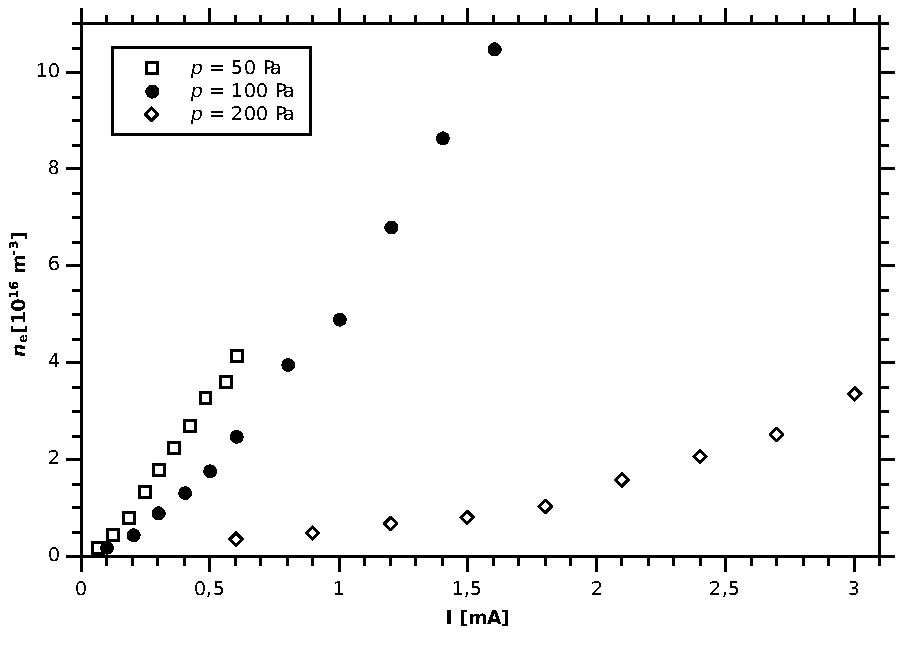
\includegraphics[width=14cm]{Graph1.pdf}
\caption{Závislost elektronových koncentrací určených relativní metodou na výbojovém proudu pro různé tlaky}
\label{graph1}
\end{center}
\end{figure}

\section{Závěr}
Měření bylo úspěšné, podařilo se naměřit vývoj elektronové koncentrace v~závislosti na výbojovém proudu pro různé tlaky. Bohužel dvě použité metody dávají rozdílné výsledky. Hodnoty získané použitím geometrických parametrů rezonátoru jsou asi $6\times$ menší než výsledky získané relativní metodou kalibrace pomocí teflonu. To si vysvětluji jednak možnou chybou při měření poloměru reaktoru a výbojové trubice a také tím, že v~rezonátoru pravděpodobně nepřevažoval očekávaný vid TM$_{010}$. Naměřené výsledky vývoje elektronové koncentrace odpovídají očekáváním, elektronová koncentrace roste přibližně lineárně s proudem (očekáváme $\vec{j} = n_\mathrm{e} e <\vec{v_\mathrm{e}}>$).


\end{document}
